\documentclass[10pt,a4paper]{article}
\usepackage[margin=2.0cm]{geometry}
\usepackage{amsmath,amssymb}
\usepackage{graphicx}
\usepackage{longtable,booktabs,pdflscape}
\usepackage[hidelinks]{hyperref}
\usepackage{url}
\usepackage{fontspec}
\setmainfont{DejaVu Serif}
\setmonofont{DejaVu Sans Mono}[Scale=0.85]
\setlength{\parskip}{4pt}
\setlength{\parindent}{0pt}
\graphicspath{{./}}
\setcounter{section}{-1}
\begin{document}
\title{v7 cloning campaign: pre-training, in-sample optimization and held-out generalization}
\author{}\date{2026-09-08}
\maketitle

State of the results on 2026-09-08. Every number in this report is read from a file of the
pulled runs (\path{~/Documents/Research/xcquinox-results/runs/dfs_step7/}) or from a CSV the figure
suite wrote beside the figure it belongs to; the file is named at each table. The figures are the
tracked sets under \path{notebooks/analysis/figures_dfs_step7_*}; the validation-best checkpoint
channel is used for every optimization figure unless a caption says otherwise.

\section{Scope and inventory}

The v7 campaign trains one network pair (an exchange network and a correlation network) per
architecture and per training-subset size, in three groups that share one protocol and differ
in their architecture axis. Each group runs its own pre-training (the cloning of the parent
functional), a fidelity certificate that gates the group's training array, and the training
array itself, one cell per (architecture, subset size).

\begin{small}
\begin{longtable}{p{0.19\linewidth}p{0.19\linewidth}p{0.19\linewidth}p{0.19\linewidth}p{0.19\linewidth}}
\toprule Group & Configuration file & Architectures & Cells done / planned & Run \\ \midrule \endhead
G1 (size) & \path{dfs_step7.dfs6311_grid3_v7g1_size.yaml} & shallow, shallow\_attn, medium, medium\_attn & medium 11/11, medium\_attn 7/11, shallow 0/11, shallow\_attn 0/11 & \path{run_20260902T145245Z} \\
G2a (descriptor families, GGA core) & \path{dfs_step7.dfs6311_grid3_v7g2a_families_core.yaml} & deep\_3x16, deep\_attn\_3x16, deep\_cusp\_3x16 & deep\_3x16 10/11, deep\_attn\_3x16 0/11, deep\_cusp\_3x16 0/11 & \path{run_20260902T145247Z} \\
G2 (descriptor families, meta-GGA) & \path{dfs_step7.dfs6311_grid3_v7g2_families_mgga.yaml} & deep\_cusp\_mgga\_3x16, deep\_mgga\_3x16, deep\_mgga\_attn\_3x16, deep\_rung35\_mgga\_3x16, deep\_rung35ms\_mgga\_3x16 & 0/55 (the first certificate reads FAIL, Sec. 2.4; the other four are pending) & \path{run_20260902T145250Z} \\
\bottomrule \end{longtable}
\end{small}

The subset-size axis is 1, 2, 3, 4, 5, 6, 7, 12, 15, 18 and 26 training molecules, drawn from
the 26-point DFS training pool by the Jensen-Shannon subset selection; the subset memberships are
printed in the footer of the held-out energy figure (Fig. 4.1). Basis 6-311++G(3df,2pd), grid
level 3, density fitting on, for every stage (\path{fidelity_certificate.json}, keys \path{basis},
\path{grid_level}, \path{density_fit}). The cells that have not finished are the attention and cusp
architectures at the larger subsets and the whole meta-GGA group; they appear as "pending" in
the tables below and are absent from the figures. Two arms of a follow-up (the 25-cycle SCF arm
and the dpyscf-parity arm, both on the medium architecture) were submitted on 2026-09-08 and
carry no results yet.


\section{Model, descriptors and the functional form}

Sources: \path{xcquinox/alec/networks.py} (the two networks), \path{xcquinox/alec/descriptors.py} and
\path{xcquinox/alec/metagga.py} (the extra descriptors), \path{xcquinox/net.py} (the attention block),
\path{xcquinox/alec/config.py} (the architecture registry). The coordinate convention is the DFS one
(\path{model.descriptor_coordinates: dfs} in every v7 file), following Dick and Fernandez-Serra,
PRB 104, L161109 (2021), whose equation numbers are quoted as "DFS Eq. n".

\subsection{Density variables}

With $n = n_\alpha + n_\beta$ the total density and $\sigma = |\nabla n|^2$,

\[
k_F = (3\pi^2 n)^{1/3}, \qquad
s = \frac{|\nabla n|}{2 k_F n}, \qquad
r_s = \left(\frac{3}{4\pi n}\right)^{1/3}, \qquad
\zeta = \frac{n_\alpha - n_\beta}{n}, \qquad
\phi(\zeta) = \tfrac12\left[(1+\zeta)^{4/3} + (1-\zeta)^{4/3}\right].
\]

$s$ is the reduced density gradient (DFS Eq. 5), $\phi$ the spin-scaling factor of DFS Eq. 4
($\phi = 1$ at $\zeta = 0$, $2^{1/3}$ at full polarization). The density is floored at the
network's \path{lower_rho_cutoff} before any of these is formed.

\subsection{Network coordinates (DFS coordinates)}

The exchange network reads one coordinate at the GGA level and two at the meta-GGA level; the
correlation network reads three and four. They are logarithmic compressions of the variables
above (DFS Eqs. 7 to 10):

\[
x_0 = \ln\!\left(n^{1/3} + 10^{-5}\right), \qquad
x_1 = \ln \phi(\zeta), \qquad
x_s = \left(1 - e^{-s^2}\right)\ln(s + 1), \qquad
x_\alpha = \ln\frac{\alpha + 1}{2}.
\]

Exchange input: $[x_s, \ldots]$, where $s$ is that of the doubled spin channel $2 n_\sigma$ (the
exchange network is evaluated per spin channel, Sec. 1.4). Correlation input:
$[x_0, x_1, x_s, \ldots]$ on the total density. The ellipsis holds the extra descriptors of the
architecture, in the registry's list order; on the meta-GGA rung the raw $\alpha$ column among
them is replaced by $x_\alpha$.

\subsection{Extra descriptors}

\textbf{Iso-orbital indicator (meta-GGA rung, \path{metagga})}, SCAN's $\alpha$ (Sun, Ruzsinszky and
Perdew, PRL 115, 036402 (2015), Eq. 2; DFS Eq. 6):

\[
\alpha = \frac{\tau - \tau_W}{\tau_{\rm unif}}, \qquad
\tau = \tfrac12 \sum_i |\nabla\psi_i|^2 = \tfrac12 \sum_{\mu\nu} P_{\mu\nu}\, \nabla\chi_\mu\cdot\nabla\chi_\nu, \qquad
\tau_W = \frac{|\nabla n|^2}{8n}, \qquad
\tau_{\rm unif} = \tfrac{3}{10}(3\pi^2)^{2/3} n^{5/3}.
\]

$\tau$ is a contraction of the live one-particle density matrix $P$ against the AO gradients,
so it is self-consistent and differentiable through the SCF without second derivatives. The
bound $\alpha \ge 0$ (the von Weizsacker inequality) is imposed by a smooth positive part rather
than a hard clip, so the descriptor and its derivative stay continuous where a spin channel holds
one orbital.

\textbf{Nuclear cusp pair (\path{cusp})}, two bounded features per grid point:

\[
x_4 = \exp(-2 Z_{\rm nearest}\, r_{\min}), \qquad
x_5 = \tanh\!\left(\frac{1}{5}\ln \sum_A \frac{Z_A}{r_A}\right).
\]

$x_4$ is a proximity feature following the density-form cusp envelope $e^{-2Zr}$ (Steiner, J.
Chem. Phys. 39, 2365 (1963), the density counterpart of Kato's wavefunction cusp); $x_5$ is the
log-compressed bare-nuclear potential $-V_{\rm ext}$, the log and the $1/5$ scale being the
conditioning of this work. Both are geometric, so the synthetic pre-training mesh (Sec. 2.1)
carries no values for them.

The remaining registry descriptors (density-matrix statistics, the rung-3.5 occupancies) are
not on any v7 axis and are not described here.

\subsection{The functional form}

Each network is a multilayer perceptron with GELU activations, \path{depth} hidden layers of \path{nodes}
units, a final linear layer (initialized at zero in the \path{deep_*} family,
\path{zero_init_final_layer}), and an output squash.
With $g$ the MLP output at a grid point,

\[
F_x = 1 + \mathcal{L}_{1.804}\!\left(G_x \cdot g_x\right), \qquad
F_c = 1 + \mathcal{L}_{2}\!\left(G_c \cdot g_c\right), \qquad
\mathcal{L}_{\lambda}(z) = \lambda\,\mathrm{sigmoid}\!\left(z - \ln(\lambda - 1)\right) - 1.
\]

$\mathcal{L}_\lambda(0) = 0$, so a zero MLP output returns $F = 1$ (the local density
approximation), and $F$ stays in $(0, \lambda)$ for every $z$. $\mathcal{L}_\lambda$ is the
DFS $I_a$ map (DFS Eq. 11) to machine precision. For exchange $\lambda = 1.804 = 1 +
\kappa\_{\rm PBE}$, the PBE Lieb-Oxford-motivated ceiling (PBE, PRL 77, 3865 (1996), Eq. 14);
DFS uses 1.174 (the tighter bound of Perdew, Ruzsinszky, Sun and Burke, J. Chem. Phys. 140,
18A533 (2014)), and the v7 meta-GGA architectures keep 1.804 as well
(\path{config.resolved_xnet_lob_lim}), a recorded deviation. For correlation $\lambda = 2$ is the
symmetric sigmoid of DFS Eq. 13; its purpose is $F_c \ge 0$, the upper value 2 is incidental.

$G$ is the uniform-electron-gas gate that pins $F = 1$ where the gradient vanishes:

\[
G = \tanh^2(s) \ \ \text{(GGA rung)}, \qquad
G = x_s + \tanh^2(x_\alpha) \ \ \text{(meta-GGA rung, DFS Eq. 12)},
\]

evaluated on the raw $s$ (and $\alpha$), never on the compressed coordinate. On the meta-GGA
rung the same gate form is used for both networks (DFS's correlation gate applies $\tanh$ to
$x_s$; recorded deviation).

The exchange-correlation energy is assembled with the exchange spin-scaling relation of
Oliver and Perdew (PRA 20, 397 (1979)) and the PW92 correlation baseline:

\[
E_{xc} = \tfrac12\left(E_x[2 n_\alpha] + E_x[2 n_\beta]\right) + E_c[n_\alpha, n_\beta], \qquad
E_x[n] = \int n\, \epsilon_x^{\rm LDA}(n)\, F_x\, d^3r, \qquad
E_c = \int n\, \epsilon_c^{\rm PW92}(r_s, \zeta)\, F_c\, d^3r,
\]

so the exchange network sees each spin channel at its doubled density (its $x_s$ is that of
$2 n_\sigma$), and the correlation network sees the total density with $\zeta$ through $x_1$.

\textbf{Attention variants.} In the \path{_attn} architectures a self-attention block (Vaswani et al.,
2017, Eqs. 1 and 2, pre-layer-norm as in Xiong et al., 2020) sits after the first hidden layer.
The hidden vector of $H$ units at a grid point is treated as $h$ tokens of dimension $d_k = H/h$
and attention runs across the token axis,

\[
\mathrm{Attn}(Q, K, V) = \mathrm{softmax}\!\left(\frac{QK^{\top}}{\sqrt{d_k}}\right) V, \qquad
x \leftarrow x + W^{O}\,\mathrm{Concat}(\mathrm{head}_1, \ldots, \mathrm{head}_h)(\mathrm{LN}(x)).
\]

It is a per-point re-mixing of hidden units, not a spatial or non-local operation.

\subsection{Architectures on the v7 axes}

\begin{landscape}
\begin{tiny}
\begin{longtable}{p{0.13\linewidth}p{0.13\linewidth}p{0.13\linewidth}p{0.13\linewidth}p{0.13\linewidth}p{0.13\linewidth}p{0.13\linewidth}}
\toprule Architecture & Rung, parent & Hidden layers x units & Attention heads & Extra descriptors & Exchange input & Correlation input \\ \midrule \endhead
shallow & GGA, PBE & 2 x 8 & none & none & $x_s$ & $x_0, x_1, x_s$ \\
shallow\_attn & GGA, PBE & 2 x 8 & 2 & none & $x_s$ & $x_0, x_1, x_s$ \\
medium & GGA, PBE & 3 x 16 & none & none & $x_s$ & $x_0, x_1, x_s$ \\
medium\_attn & GGA, PBE & 3 x 16 & 4 & none & $x_s$ & $x_0, x_1, x_s$ \\
deep\_3x16 & GGA, PBE & 3 x 16 & none & none & $x_s$ & $x_0, x_1, x_s$ \\
deep\_attn\_3x16 & GGA, PBE & 3 x 16 & 4 & none & $x_s$ & $x_0, x_1, x_s$ \\
deep\_cusp\_3x16 & GGA, PBE & 3 x 16 & none & cusp & $x_s, x_4, x_5$ & $x_0, x_1, x_s, x_4, x_5$ \\
deep\_cusp\_mgga\_3x16 & meta-GGA, SCAN & 3 x 16 & none & cusp, $\alpha$ & $x_s, x_4, x_5, x_\alpha$ & $x_0, x_1, x_s, x_4, x_5, x_\alpha$ \\
\bottomrule \end{longtable}
\end{tiny}
\end{landscape}

medium and deep\_3x16 share the layer geometry; the \path{deep_*} family carries the
physics-correction flags of the registry (\path{dm_entropy_intensive}, \path{descriptor_log_transform},
\path{zero_init_final_layer}), of which only the zero initialization and the cusp column-1 logarithm
act on this axis (the DFS coordinates already compress $s$). All v7 networks are unanchored
(\path{model.parent_anchor: false}): the network output is the whole enhancement factor, and the
parent functional enters only as the pre-training target.


\section{Pre-training (functional cloning)}

Sources: \path{xcquinox/alec/pretrain.py}, \path{xcquinox/alec/pretrain_data_gen.py}, the \path{pretrain:} and
\path{fidelity:} blocks of the resolved configurations, \path{pretrain/<arch>/pretrain_metadata.json} and
\path{pretrain/<arch>/fidelity_certificate.json} of each run.

\subsection{Set, targets and objective}

Each network is fitted to reproduce its parent functional's enhancement factor pointwise on the
parent's own self-consistent densities: PBE for the GGA rung, SCAN for the meta-GGA rung. The set
is the DFS pre-training inventory (8 free atoms and 22 G2/97 molecules at the GGA level; 20
molecules at the meta-GGA level, which drops H2 and N2) plus every single-atom species of the
BH76 and W4-11 pools at its production charge and spin (the 12 neutral elements and the F- and
Cl- anions), 39 systems for the GGA groups and 38 for the meta-GGA group (\path{n_systems} of the
certificates). The targets are stored per grid point as

\[
t_x = F_x^{\rm parent} - 1 = \frac{\epsilon_x^{\rm parent}}{\epsilon_x^{\rm LDA}} - 1, \qquad
t_c = F_c^{\rm parent} - 1 = \frac{\epsilon_c^{\rm parent}}{\epsilon_c^{\rm PW92}} - 1,
\]

from spin-resolved libxc evaluations, the exchange rows posed per spin channel at the doubled
density $(2 n_\sigma, 4\sigma_{\sigma\sigma})$, the footing the production exchange evaluates
(\path{exchange_footing: spin_channel}). A synthetic $(r_s, s, \alpha)$ mesh (the DFS SI's $(s,
\alpha)$ grid extended to three dimensions) is added as a regularizer at a fixed 30 percent share
of the integration weight (\path{mesh_fraction: 0.3}); its rows belong to no system.

The objective per network is the integration-weighted pointwise residual plus a per-system
energy term (\path{_PretrainLoss}):

\[
\mathcal{L}_{\rm pre} = \frac{\sum_i w_i\,(F_i^{\rm NN} - 1 - t_i)^2}{\sum_i w_i}
\;+\; w_E\,\frac{1}{N_{\rm sys}}\sum_{s}\Big(\sum_{i\in s} w^{\rm grid}_i\, n_i\,\epsilon_i^{\rm LDA}\, F_i^{\rm NN} - E_{xc,s}^{\rm parent}\Big)^2,
\qquad w_i = |n_i\, \epsilon_i^{\rm LDA}|\, w_i^{\rm grid}, \quad w_E = 0.1 .
\]

The energy term exists because the pointwise residual alone does not bound a system's energy:
across the earlier campaign the architecture with the lowest exchange residual carried the
largest atomization-energy offset from its parent. Schedule: Adam, 20000 steps, learning rate
$10^{-3}$ decaying linearly to $10^{-5}$ from the midpoint, gradient clip 1.0, a 20 percent
held-out validation slice scored every 50 steps with patience 300 checks (\path{pretrain:} block).
The curves of Fig. 2.1 are the pointwise term per step taken.

\subsection{The fidelity certificate}

After the fit, the saved networks are re-evaluated on every system of the set at the production
basis and grid and compared with the parent: the per-system exchange-correlation energy error
$\Delta E_{xc,s} = E_{xc,s}^{\rm NN} - E_{xc,s}^{\rm parent}$, and, for every molecule, the
atomization-energy error $\Delta AE = \Delta E_{xc,{\rm mol}} - \sum_A \Delta E_{xc,A}$ against
the parent's own atomization energy. The gate (\path{fidelity:} block, two-tier since 2026-09-02) is

\[
\max_{\rm atoms} |\Delta E_{xc,A}| \le 1.0\ \text{mHa}, \qquad
\mathrm{mean}_{\rm mol} |\Delta AE| \le 1.0\ \text{kcal/mol}, \qquad
\max_{\rm mol} |\Delta AE| \le 2.0\ \text{kcal/mol},
\]

and a failing certificate makes the pre-training task exit without success, which holds the
group's preflight and training array. The certificate is what makes the training-stage
comparison against PBE (or SCAN) meaningful: every trained cell starts from a network that is
its parent to within these tolerances.

\subsection{Figures}

\textbf{Fig. 2.1} Pre-training loss curves, X-net (exchange) and C-net (correlation), one line per
architecture, log-y; the spikes are the validation checks' snapshot reloads.

\begin{center}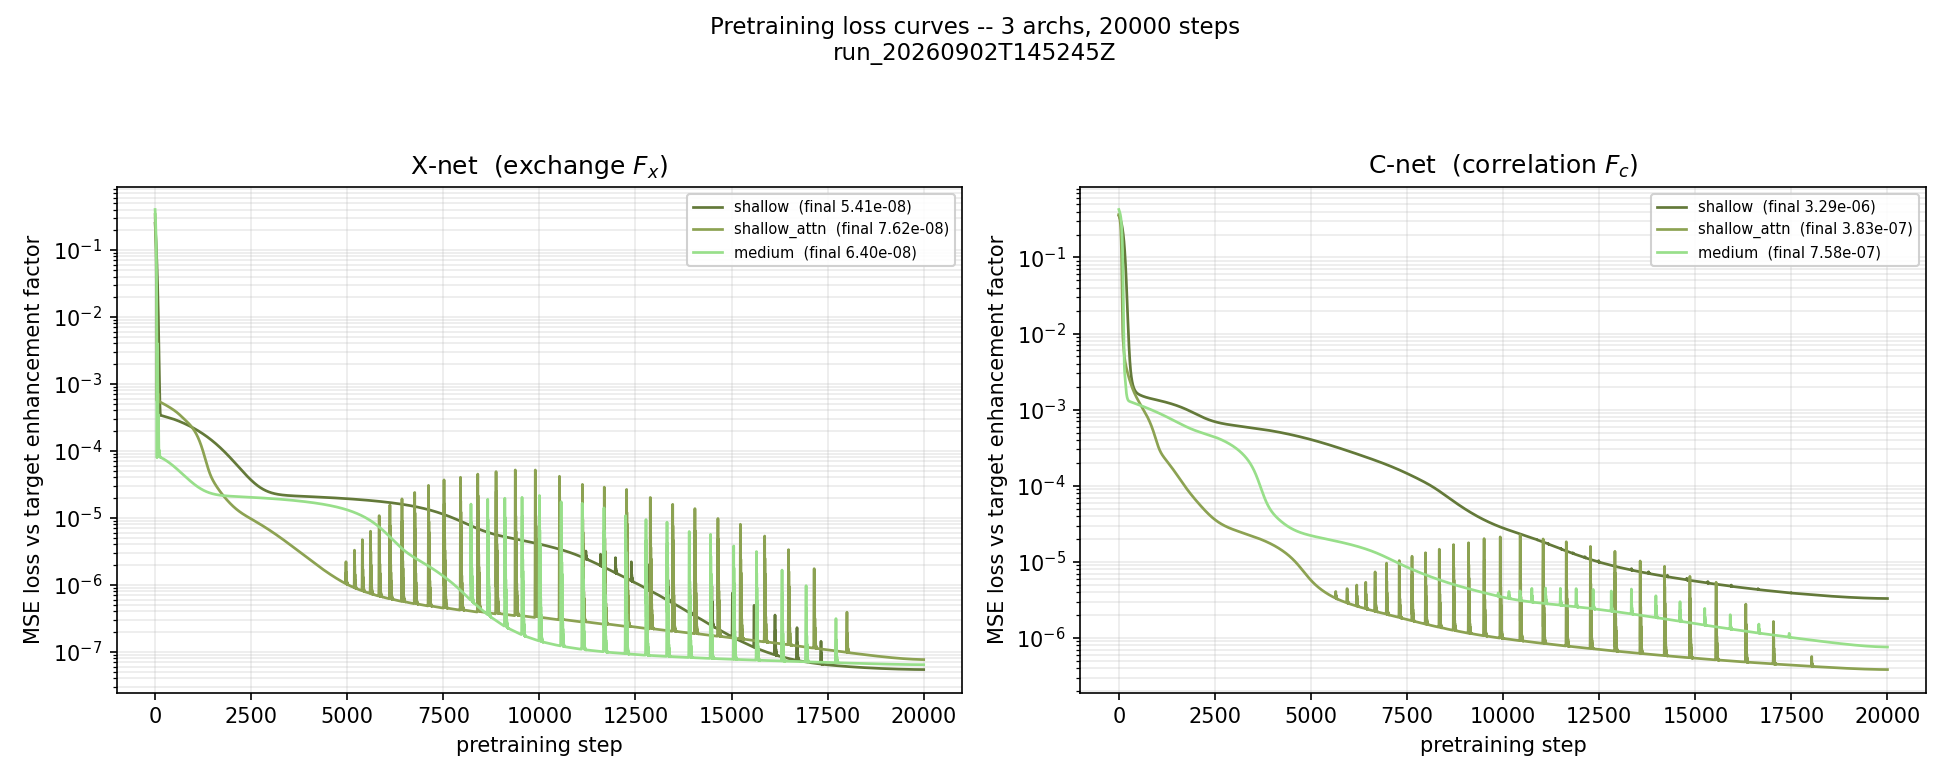
\includegraphics[width=\linewidth]{figures_dfs_step7_v7_pretrain/pretrain_curves_v7g1_size.png}\end{center}

\begin{center}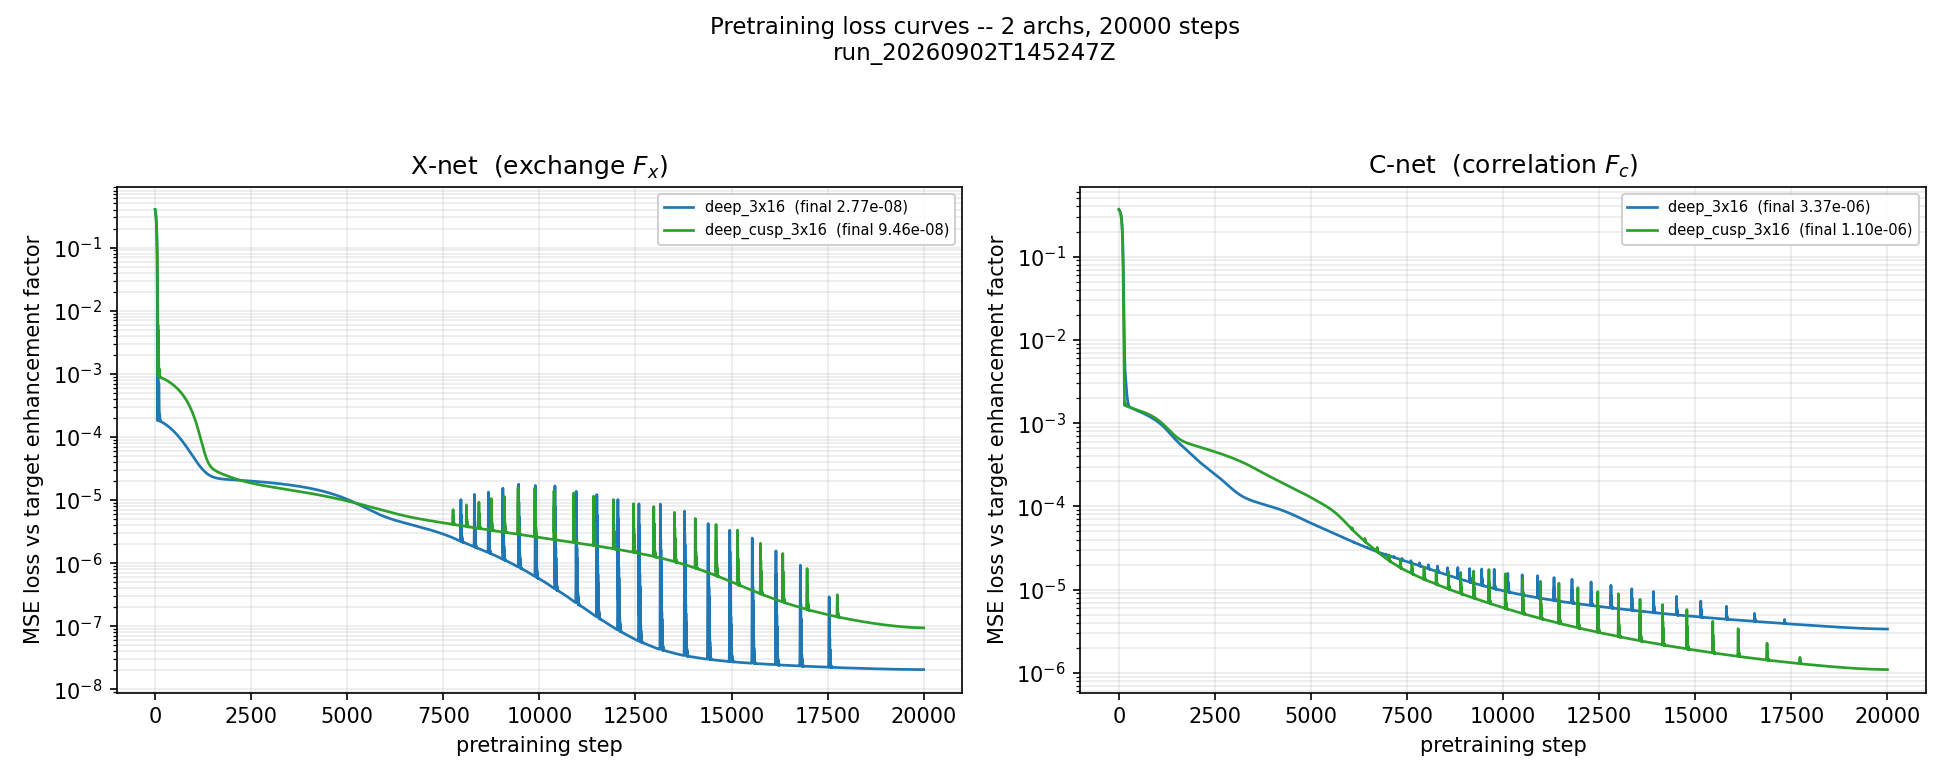
\includegraphics[width=\linewidth]{figures_dfs_step7_v7_pretrain/pretrain_curves_v7g2a_families_core.png}\end{center}

\begin{center}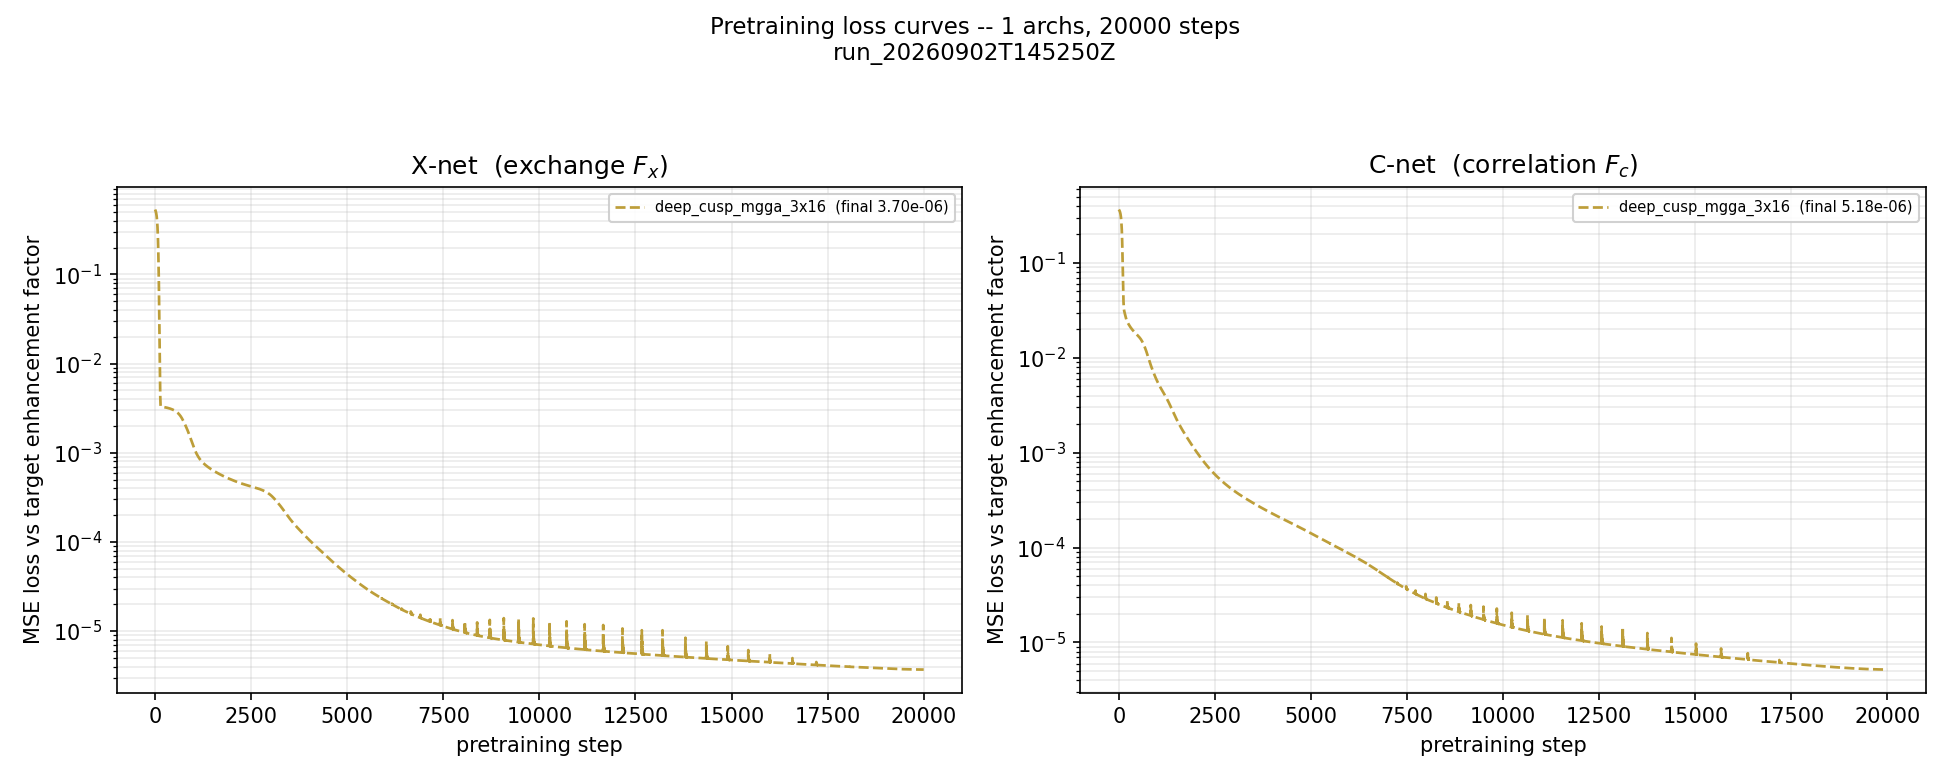
\includegraphics[width=\linewidth]{figures_dfs_step7_v7_pretrain/pretrain_curves_v7g2_families_mgga.png}\end{center}

\textbf{Fig. 2.2} Certificate summary: mean $|\Delta AE|$ per architecture (bar) with the
per-species maximum (marker), against the 1.0 kcal/mol mean gate and the 2.0 kcal/mol
per-species backstop; the v7 round beside the legacy (pre-protocol, single-tolerance) round of
the same G1 architectures. The meta-GGA certificate is tabulated in Sec. 2.4 (the summary figure
was rendered before it existed).

\begin{center}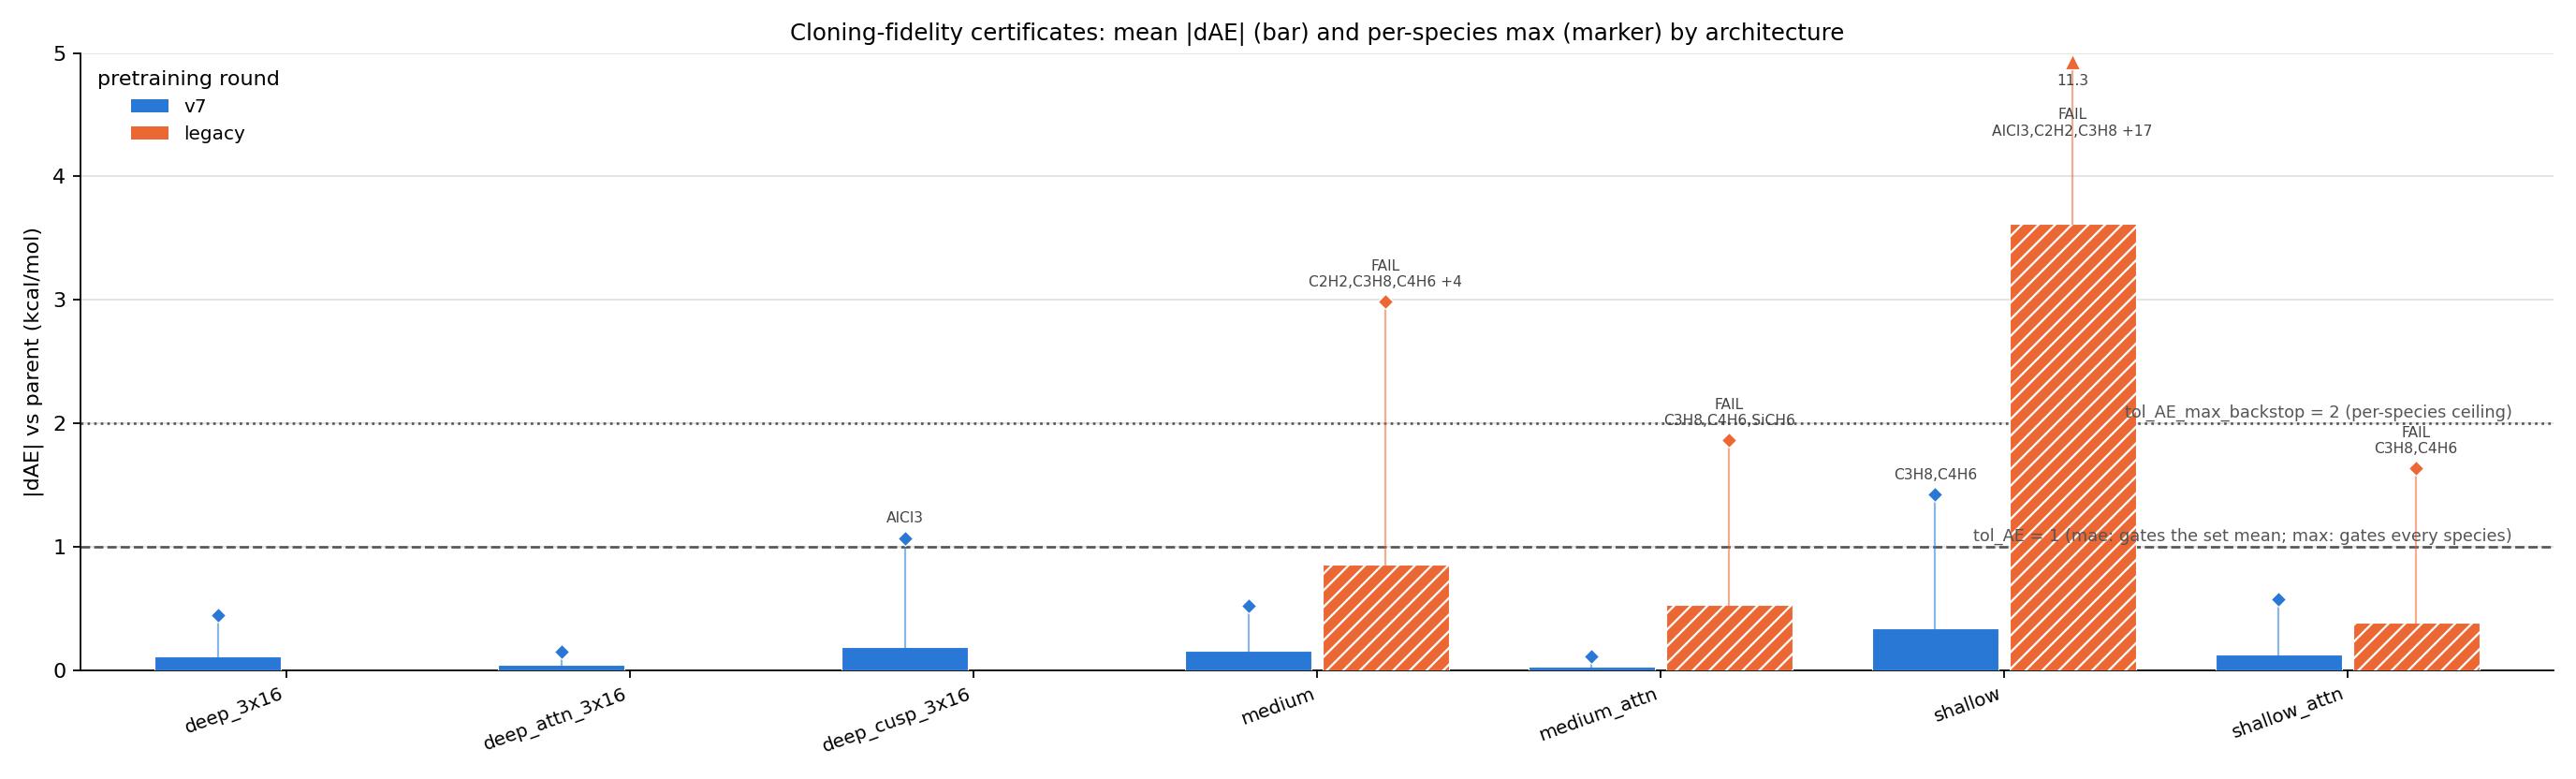
\includegraphics[width=\linewidth]{figures_dfs_step7_v7_pretrain/certificate_summary_v7.png}\end{center}

\textbf{Fig. 2.3} Pre-trained enhancement factors against the parent, per architecture: $F_x(s)$ at
$n = 1$ and $F_c(s; r_s)$ at $\zeta = 0$, $r_s \in \{0.5, 2, 5\}$, with the difference panels
$F^{\rm NN} - F^{\rm parent}$. For the meta-GGA clone the slices are at $\alpha = 0$ and
$\alpha = 1$ (the SCAN Fig. 1 convention). The parent curves are the anchor's own libxc-constant
implementations.

\begin{center}
\includegraphics[width=\linewidth]{figures_dfs_step7_v7_pretrain/fx_fc_v7g1_size/pretrain_fx_fc_medium.png}\end{center}

\begin{center}
\includegraphics[width=\linewidth]{figures_dfs_step7_v7_pretrain/fx_fc_v7g1_size/pretrain_fx_fc_medium_attn.png}\end{center}

\begin{center}
\includegraphics[width=\linewidth]{figures_dfs_step7_v7_pretrain/fx_fc_v7g2a_families_core/pretrain_fx_fc_deep_3x16.png}\end{center}

\begin{center}
\includegraphics[width=\linewidth]{figures_dfs_step7_v7_pretrain/fx_fc_v7g2_families_mgga/pretrain_fx_fc_deep_cusp_mgga_3x16.png}\end{center}

\textbf{Fig. 2.4} The learned corrections of every GGA architecture on one axis (G1 and G2a).

\begin{center}
\includegraphics[width=\linewidth]{figures_dfs_step7_v7_pretrain/fx_fc_v7g1_size/pretrain_fx_fc_delta_all.png}\end{center}

\begin{center}
\includegraphics[width=\linewidth]{figures_dfs_step7_v7_pretrain/fx_fc_v7g2a_families_core/pretrain_fx_fc_delta_all.png}\end{center}

The shallow pair and the deep\_attn\_3x16 and deep\_cusp\_3x16 clones are drawn in the same
directories (\path{pretrain_fx_fc_<arch>.png}).

\subsection{Certificate results}

Read from \path{pretrain/<arch>/fidelity_certificate.json} and \path{pretrain_metadata.json}; the
pointwise losses are the saved network's, in units of the squared enhancement-factor residual.


\begin{landscape}
\begin{tiny}
\begin{longtable}{llllllllll}
\toprule Group & Architecture & Parent & Steps & Pointwise loss X / C & max atom $\lvert\Delta E_{xc}\rvert$ (mHa) & mean $\lvert\Delta AE\rvert$ (kcal/mol) & max $\lvert\Delta AE\rvert$ (kcal/mol) & Species over 1 kcal/mol & Verdict \\ \midrule \endhead
G1 & shallow & PBE & 20000 & 5.41e-08 / 3.29e-06 & 0.369 & 0.343 & 1.421 & C3H8, C4H6 & PASS \\
G1 & shallow\_attn & PBE & 20000 & 7.62e-08 / 3.83e-07 & 0.201 & 0.131 & 0.573 & none & PASS \\
G1 & medium & PBE & 20000 & 6.40e-08 / 7.58e-07 & 0.210 & 0.162 & 0.519 & none & PASS \\
G1 & medium\_attn & PBE & 20000 & 1.51e-08 / 6.70e-08 & 0.058 & 0.031 & 0.115 & none & PASS \\
G2a & deep\_3x16 & PBE & 20000 & 2.77e-08 / 3.37e-06 & 0.439 & 0.114 & 0.450 & none & PASS \\
G2a & deep\_attn\_3x16 & PBE & 20000 & 1.48e-08 / 9.86e-08 & 0.123 & 0.042 & 0.149 & none & PASS \\
G2a & deep\_cusp\_3x16 & PBE & 20000 & 9.46e-08 / 1.10e-06 & 0.439 & 0.188 & 1.071 & AlCl3 & PASS \\
G2 & deep\_cusp\_mgga\_3x16 & SCAN & 20000 & 3.70e-06 / 5.18e-06 & 3.132 & 2.062 & 7.257 & AlCl3, C2H2, C3H8, C4H6, CH2, CH4, CO, CO2, F2, H2O, HCN, O2, PH3, SiCH6 & FAIL \\
\bottomrule \end{longtable}
\end{tiny}
\end{landscape}


Every GGA clone passes on all three criteria; the two with a species above 1 kcal/mol (shallow:
C3H8, C4H6; deep\_cusp\_3x16: AlCl3) pass on the mean and under the 2.0 kcal/mol backstop. The
attention variants are the tightest clones by every measure (medium\_attn: max atom 0.058 mHa,
mean 0.031 kcal/mol; deep\_attn\_3x16: 0.123 mHa, 0.042 kcal/mol), at the price of the longest
fits (about 28 h against 3.6 to 3.8 h for their plain twins, \path{duration_seconds}).

The meta-GGA clone deep\_cusp\_mgga\_3x16 fails all three criteria after a converged 20000-step
fit (pointwise residuals 3.7e-6 and 5.2e-6, an order of magnitude above the GGA clones'): the
largest free-atom error is 3.13 mHa (O; B 2.91, Be 2.61), the mean atomization error 2.06
kcal/mol and the largest 7.26 kcal/mol (C4H6; C3H8 7.19, O2 4.77, SiCH6 3.52, CH4 3.47), 14 of
22 molecules above 1 kcal/mol, every one of the eight largest errors of the same sign. Fig. 2.3
(bottom) shows where the clone misses SCAN: the $\alpha = 0$ exchange slice is 0.015 to 0.027
above SCAN for $s > 2$ and the $\alpha = 1$ correlation slices sit 0.01 to 0.03 below it at
$r_s = 0.5$, systematic offsets that do not cancel between a molecule and its atoms. The v6
meta-GGA certificates, all PASS, were fitted in the anchored model class (the network learns a
correction on top of SCAN); this is the first unanchored meta-GGA clone the two-tier gate has
judged. The four remaining meta-GGA architectures are pending; whether the rung or this
architecture is the cause is decided by their certificates. Until then the meta-GGA training
array is held.


\section{Optimization, in-sample}

Sources: \path{xcquinox/alec/losses.py} (\path{L5_gradnorm_vxc_step7}, the channel terms),
\path{xcquinox/alec/train.py} (the per-molecule loop, the optimizer), \path{xcquinox/alec/oneshot.py}
(the SCF tail window), \path{xcquinox/alec/solver_manual.py} (the differentiable SCF), the
\path{hyperparams:} and \path{solvers:} blocks of the resolved configurations, and per cell
\path{train_metadata.json}, \path{losses.npy}, \path{aux_log.pkl}, \path{eval/per_molecule.json}.

\subsection{Training protocol}

Each cell trains the certified clone of its architecture on a subset of the 26-point DFS pool.
The per-molecule update scheme takes one optimizer step per training group (a reaction, or a
molecule with its density and potential references) per epoch, so an epoch is one pass over
the groups. The loss of a group is the fixed weighted sum

\[
\mathcal{L} = 1\cdot\mathcal{L}_{AE} + 1\cdot\mathcal{L}_{\rm rxn} + 1\cdot\mathcal{L}_{IP} + 1\cdot\mathcal{L}_{v_{xc}} + 20\cdot\mathcal{L}_{\rho},
\]

the Letter's $\lambda_{RE} = 1$, $\lambda_n = 20$ structure (\path{effective_channel_weights}; the
GradNorm balancer is configured but dormant under this scheme, and the \path{vxc_weight} 0.01 and
\path{density_weight} 0.1 pre-scales are forced to 1). The channels, with $E^{\rm NN}$ the
self-consistent total energy of the 3-cycle SCF (Sec. 3.2) and $t = 0, \ldots, N-1$ the cycle
index:

\begin{itemize}
\item Reaction energies (\path{ae_as_reactions: true} routes the W4-11 atomizations here as molecule-to-atoms reactions with the network's own atoms, beside the BH76 barriers): \[ \mathcal{L}_{\rm rxn} = \frac{1}{|T|}\sum_{t\in T} w_t^2\, r_t^2, \qquad r_t = \sum_i c_i\, E^{\rm NN}_{i,t} - E^{\rm ref}, \qquad w_t = \left(\frac{t}{N-1}\right)^2, \] $T$ the kept SCF tail (the last $\min(N, 10)$ cycles; at $N = 3$ all three, $w_t^2 = 0, 1/16, 1$), the DFS convergence-tail scoring (DFS Eqs. 15 and 16) that penalizes a non-converging SCF instead of one arbitrary final cycle. Absolute Ha$^2$ (\path{loss_metric: absolute}). References: W4-11 atomization energies and the W2-F12 BH76 barrier heights of GMTKN55.
\item Atom anchors (the residue of the AE channel once the atomizations are reactions): the free atoms of the subset are held near their exact non-relativistic energies $E_Z^{\rm anchor}$ (Chakravorty et al., PRA 47, 3649 (1993)), $\mathcal{L}_{AE} = 0.01\cdot\mathrm{mean}_Z\, (E_Z^{\rm NN} - E_Z^{\rm anchor})^2 / (E_Z^{\rm anchor})^2$.
\item Ionization potentials, $\mathcal{L}_{IP} = \mathrm{mean}\,(E^{\rm NN}_{+} - E^{\rm NN}_0 - IP^{\rm ref})^2$, present in the form but empty on every v7 subset (no IP13 point is selected).
\item Exchange-correlation potential, on the reference density (frozen features): $\mathcal{L}_{v_{xc}} = \|V_{xc}^{\rm NN} - V_{xc}^{\rm ref}\|_F^2 / n_{\rm AO}^2$, summed over spin channels for open shells.
\item Density, the final mixed density of the SCF against the CCSD reference density on the same grid, per electron squared (the Letter's Eq. 17 normalization; \path{density_per_electron: true}): \[ \mathcal{L}_{\rho} = \mathrm{mean}_{\rm mol}\,\frac{\sum_g w_g\,(n^{\rm NN}_g - n^{\rm ref}_g)^2}{N_e^2}, \qquad N_e = \sum_g w_g\, n^{\rm ref}_g . \]
\end{itemize}

Optimizer: AdamW, learning rate $10^{-3}$ held for the first half of the run and decayed
linearly to $10^{-5}$ over the second (\path{lr_decay_start: 0.5}), weight decay $10^{-4}$, gradient
clip 1.0. 200 epochs (\path{n_steps}), a validation reaction-energy MAE on the 47-reaction validation
slice every 25 epochs, early stop after 5 checks without a 0.1 kcal/mol improvement; three
checkpoints are kept (final, lowest training loss, lowest validation MAE), and the figures of
Secs. 3 and 4 read the validation-best one. Over the 18 G1 cells the runs took 150 to 200
epochs (early-stopped in 12) and 1.2 to 22 h of wall each (\path{train_metadata.json}).

\subsection{The differentiable SCF}

The energies and densities above are self-consistent: the manual backend runs a fixed
$N = 3$ cycles from the converged PBE density (\path{solver: full_3}), diagonalizing the Kohn-Sham
matrix built from the network's $V_{xc}$ each cycle, with the DFS decaying linear mixing
$D_{t+1} = (1 - a_t) D_t + a_t D^{\rm out}_t$, $a_t = 0.3^{t} + 0.3$, a freeze once
$|\Delta E| < 10^{-6}$ Ha, and gradients through every cycle. The density scored by
$\mathcal{L}_\rho$ and by the density metrics is the last mixed density; three cycles do not
converge the SCF for a functional far from a fixed point, which is the subject of the two arms
submitted on 2026-09-08 (25 cycles; dpyscf parity) and of the converged-SCF re-evaluation in
flight. The 2026-09-07 audit (\path{notebooks/analysis/AUDIT_2026-09-01.md}, the density section)
records the full parity table against dpyscf.

\subsection{Figures}

\textbf{Fig. 3.1} Per-channel training losses, one figure per architecture: the total and the
five channels at their trained weights as per-epoch means (log y; the five panels add up to
the total), one curve per subset size, the validation-MAE checks with the validation-best
epoch starred, from each cell's \path{aux_log.pkl}.

\begin{center}
\includegraphics[width=\linewidth]{figures_dfs_step7_dfs6311_grid3_v7g1_size_val_best/training_loss_channels_medium.png}\end{center}

\begin{center}
\includegraphics[width=\linewidth]{figures_dfs_step7_dfs6311_grid3_v7g1_size_val_best/training_loss_channels_medium_attn.png}\end{center}

\begin{center}
\includegraphics[width=\linewidth]{figures_dfs_step7_dfs6311_grid3_v7g2a_families_core_val_best/training_loss_channels_deep_3x16.png}\end{center}

\textbf{Fig. 3.2} Total training loss per cell (rolling mean, log-y), the loss actually stepped.

\begin{center}
\includegraphics[width=\linewidth]{figures_dfs_step7_dfs6311_grid3_v7g1_size_val_best/training_loss_total.png}\end{center}

\begin{center}
\includegraphics[width=\linewidth]{figures_dfs_step7_dfs6311_grid3_v7g2a_families_core_val_best/training_loss_total.png}\end{center}

\textbf{Fig. 3.3} The trained enhancement factors against PBE, one curve per subset size (validation-best
checkpoint): $F_x(s)$ at $n = 1$ and $F_c(s; r_s = 2)$ at $\zeta = 0$, with the differences.
The pre-trained curve of Fig. 2.3 is the starting point of every curve here.

\begin{center}
\includegraphics[width=\linewidth]{figures_dfs_step7_dfs6311_grid3_v7g1_size_val_best/trained_fx_fc_medium.png}\end{center}

\begin{center}
\includegraphics[width=\linewidth]{figures_dfs_step7_dfs6311_grid3_v7g1_size_val_best/trained_fx_fc_medium_attn.png}\end{center}

\begin{center}
\includegraphics[width=\linewidth]{figures_dfs_step7_dfs6311_grid3_v7g2a_families_core_val_best/trained_fx_fc_deep_3x16.png}\end{center}

The training moves the exchange factor by up to 0.18 (medium, $s \approx 2.5$) and 0.14
(deep\_3x16), a systematic raise between $s = 1.5$ and 6 with a dip below 1.5, similar in shape
across subset sizes and largest at the small subsets; the correlation factor at $r_s = 2$ is
raised by 0.5 to 1.4 for $s > 1$, the cells with 1 to 3 molecules leaving $F_c$ above 1 at large
$s$. The correction is not a small perturbation of PBE, and it is what the held-out comparison
of Sec. 4 measures.

\textbf{Fig. 3.4} Training-set density against CCSD, network and PBE, per cell and per molecule
(the in-sample density fit, final checkpoint; \path{eval/per_molecule.json} exists for the final
checkpoint only).

\begin{center}
\includegraphics[width=\linewidth]{figures_dfs_step7_dfs6311_grid3_v7g1_size_val_best/insample_density_vs_ccsd.png}\end{center}

\begin{center}
\includegraphics[width=\linewidth]{figures_dfs_step7_dfs6311_grid3_v7g2a_families_core_val_best/insample_density_vs_ccsd.png}\end{center}

\textbf{Fig. 3.5} In-sample energy and density in DFS units, the 3x3 layout of Fig. 4.5 on the
training set: rows WTMAD-2 / $\varepsilon_n$ / $\mathcal{ED}$, columns BH76 / W4-11 / combined,
network against PBE on each cell's own training reactions and molecules. The energy leg is the
training reactions themselves (the W4-11 atomizations as molecule-to-atoms reactions and the
BH76 barriers of \path{train_metadata.json}), each formed from the final checkpoint's
self-consistent species energies in \path{eval/per_molecule.json} against its reference; PBE on
the same reactions from the same file's PBE energies. The dashed pooled line is the union of
the run's training reactions; the capped spans and the verdicts use each cell's own.

\begin{center}
\includegraphics[width=\linewidth]{figures_dfs_step7_dfs6311_grid3_v7g1_size_val_best/insample_by_pool_3x3_eps.png}\end{center}

\begin{center}
\includegraphics[width=\linewidth]{figures_dfs_step7_dfs6311_grid3_v7g2a_families_core_val_best/insample_by_pool_3x3_eps.png}\end{center}

\subsection{What the in-sample figures show, and one figure they must not}

The training-set density panels (Fig. 3.4) are the direct check that the density channel
trains: on the supervised molecules the cell-mean density RMSE against CCSD is below PBE's in
all 28 cells, the NN/PBE ratio 0.72 to 0.97 for medium, 0.57 to 0.76 for medium\_attn and 0.68
to 0.93 for deep\_3x16, with the weakest fits at 3 to 6 molecules and 150 of the 182 trained
species-cells improved (the table below, computed from \path{eval/per_molecule.json} with case twins
collapsed). The total loss (Fig. 3.2) falls by a factor 1.2 to 5.1 between the first and the
last 5 percent of the updates and is flat by the end, without the late instability seen in
earlier campaigns.

Per channel (Fig. 3.1; the table below gives the first and last five-epoch means of every
weighted channel and the validation checks, computed from the logs): the reaction channel
falls in every cell, by 3x (deep\_3x16 at 18 molecules) to 190x (medium\_attn at 2), and
the density channel by 1.3x to 4.6x, both settling within the first 25 epochs; the potential channel,
the extra term of the parity table, rises over training from seven molecules upward (medium
at 12: 2.2e-5 to 2.8e-5; at 18: 3.9e-5 to 4.3e-5), the anchors channel stays at 1e-7 to
1e-6 and the ionization channel (populated from 12 molecules only) peaks in the first 50
epochs and falls. The validation MAE of the 2-to-6-molecule cells of medium and deep\_3x16
rises after the first check (medium at 2: 11.7 to 32.7 kcal/mol, validation-best at epoch
25), which is the over-fitting the held-out dip of Sec. 4.5 records; the cells from seven
molecules upward hold 6 to 9 kcal/mol across their checks.

\begin{landscape}
\begin{tiny}
\begin{longtable}{llllllllllll}
\toprule Group & Architecture & Subset & Epochs & total first/last & AE first/last & reactions first/last & IP13 first/last & V\_xc first/last & rho first/last & val MAE checks (kcal/mol) & val-best epoch \\ \midrule \endhead
G1 & medium & 1 & 175 & 4.47e-05 / 3.66e-05 & 7.77e-08 / 1.93e-07 & 7.25e-07 / 4.16e-09 & 0.00e+00 / 0.00e+00 & 3.13e-05 / 2.68e-05 & 1.26e-05 / 9.62e-06 & 9.4, 8.2, 8.4, 9.1, 9.0, 9.1, 9.1 & 50 \\
G1 & medium & 2 & 150 & 1.79e-04 / 4.29e-05 & 1.66e-07 / 7.16e-07 & 1.31e-04 / 4.49e-06 & 0.00e+00 / 0.00e+00 & 1.35e-05 / 1.73e-05 & 3.43e-05 / 2.05e-05 & 11.7, 25.2, 28.1, 30.0, 31.3, 32.7 & 25 \\
G1 & medium & 3 & 150 & 1.83e-04 / 3.85e-05 & 4.91e-08 / 7.93e-08 & 1.36e-04 / 2.04e-06 & 5.12e-06 / 2.63e-06 & 1.39e-05 / 1.37e-05 & 2.82e-05 / 2.01e-05 & 14.6, 22.5, 22.0, 17.0, 16.0, 15.6 & 25 \\
G1 & medium & 4 & 200 & 1.57e-04 / 4.19e-05 & 4.50e-08 / 3.98e-08 & 1.10e-04 / 3.05e-06 & 3.94e-06 / 2.06e-06 & 1.21e-05 / 1.33e-05 & 3.12e-05 / 2.35e-05 & 18.2, 20.0, 16.6, 15.6, 15.4, 14.9, 14.7, 14.6 & 200 \\
G1 & medium & 5 & 150 & 1.39e-04 / 4.10e-05 & 3.75e-08 / 6.83e-08 & 9.16e-05 / 5.96e-06 & 1.08e-05 / 2.89e-06 & 1.07e-05 / 1.25e-05 & 2.62e-05 / 1.96e-05 & 19.2, 23.4, 23.3, 26.8, 27.6, 27.7 & 25 \\
G1 & medium & 6 & 150 & 1.34e-04 / 4.51e-05 & 2.52e-08 / 7.90e-08 & 8.98e-05 / 8.13e-06 & 7.05e-06 / 2.11e-06 & 1.01e-05 / 1.33e-05 & 2.70e-05 / 2.15e-05 & 18.4, 21.1, 21.9, 22.6, 22.2, 22.4 & 25 \\
G1 & medium & 7 & 200 & 1.58e-04 / 5.90e-05 & 1.29e-07 / 2.96e-08 & 9.01e-05 / 1.60e-05 & 8.12e-06 / 1.89e-06 & 1.69e-05 / 2.35e-05 & 4.29e-05 / 1.76e-05 & 7.8, 7.3, 7.4, 7.1, 6.9, 7.2, 6.9, 7.0 & 175 \\
G1 & medium & 12 & 200 & 2.14e-04 / 8.38e-05 & 1.03e-07 / 4.38e-08 & 1.40e-04 / 3.07e-05 & 4.65e-06 / 1.56e-06 & 2.17e-05 / 2.79e-05 & 4.78e-05 / 2.36e-05 & 9.0, 8.5, 8.3, 8.7, 8.1, 7.8, 7.9, 7.9 & 150 \\
G1 & medium & 15 & 150 & 1.96e-04 / 8.79e-05 & 1.03e-07 / 8.94e-08 & 1.15e-04 / 3.02e-05 & 4.00e-06 / 1.50e-06 & 2.92e-05 / 3.39e-05 & 4.74e-05 / 2.22e-05 & 7.3, 8.0, 7.6, 7.5, 7.9, 7.5 & 25 \\
G1 & medium & 18 & 150 & 1.94e-04 / 1.03e-04 & 1.05e-07 / 2.08e-07 & 1.08e-04 / 3.13e-05 & 3.45e-06 / 3.78e-06 & 3.92e-05 / 4.31e-05 & 4.38e-05 / 2.46e-05 & 7.1, 8.0, 7.3, 8.0, 7.2, 7.3 & 25 \\
G1 & medium & 26 & 175 & 1.79e-04 / 9.16e-05 & 1.98e-07 / 1.84e-07 & 9.34e-05 / 2.76e-05 & 3.08e-06 / 1.15e-06 & 3.73e-05 / 3.73e-05 & 4.54e-05 / 2.53e-05 & 9.3, 8.9, 9.3, 9.0, 10.4, 9.3, 9.7 & 50 \\
G1 & medium\_attn & 1 & 150 & 4.49e-05 / 2.28e-05 & 1.48e-07 / 7.30e-07 & 3.63e-07 / 1.39e-08 & 0.00e+00 / 0.00e+00 & 3.49e-05 / 1.60e-05 & 9.52e-06 / 6.03e-06 & 8.2, 13.8, 17.9, 18.7, 15.8, 17.0 & 25 \\
G1 & medium\_attn & 2 & 200 & 1.44e-04 / 2.11e-05 & 3.02e-07 / 2.63e-07 & 9.54e-05 / 5.08e-07 & 0.00e+00 / 0.00e+00 & 1.36e-05 / 1.29e-05 & 3.43e-05 / 7.44e-06 & 36.5, 31.3, 24.0, 16.9, 9.6, 7.6, 7.2, 7.2 & 200 \\
G1 & medium\_attn & 3 & 200 & 1.51e-04 / 2.30e-05 & 8.53e-08 / 2.28e-07 & 9.82e-05 / 6.22e-07 & 7.06e-06 / 3.99e-08 & 1.32e-05 / 1.37e-05 & 3.28e-05 / 8.41e-06 & 29.5, 21.7, 13.3, 15.6, 17.8, 19.4, 20.8, 21.2 & 75 \\
G1 & medium\_attn & 4 & 200 & 1.25e-04 / 2.40e-05 & 4.86e-08 / 3.67e-08 & 8.16e-05 / 1.36e-06 & 4.99e-06 / 1.87e-08 & 1.16e-05 / 1.26e-05 & 2.66e-05 / 9.94e-06 & 22.1, 12.7, 7.4, 7.3, 8.0, 7.8, 7.6, 8.1 & 100 \\
G1 & medium\_attn & 5 & 200 & 1.12e-04 / 2.00e-05 & 7.20e-08 / 7.07e-08 & 6.49e-05 / 1.49e-06 & 1.12e-05 / 4.01e-08 & 1.06e-05 / 1.09e-05 & 2.51e-05 / 7.51e-06 & 25.0, 15.4, 9.8, 9.8, 12.1, 12.7, 13.3, 13.4 & 100 \\
G1 & medium\_attn & 6 & 200 & 1.04e-04 / 2.27e-05 & 4.82e-08 / 3.52e-08 & 6.12e-05 / 2.06e-06 & 6.95e-06 / 1.19e-07 & 1.05e-05 / 1.15e-05 & 2.57e-05 / 8.98e-06 & 22.4, 19.5, 10.6, 9.9, 8.9, 8.6, 8.9, 9.0 & 150 \\
G1 & medium\_attn & 7 & 200 & 1.18e-04 / 3.43e-05 & 1.18e-07 / 1.77e-07 & 5.79e-05 / 8.12e-07 & 7.39e-06 / 4.76e-07 & 1.98e-05 / 1.98e-05 & 3.24e-05 / 1.30e-05 & 7.2, 5.9, 5.9, 5.7, 6.6, 6.5, 6.7, 6.7 & 100 \\
G2a & deep\_3x16 & 1 & 175 & 4.46e-05 / 3.20e-05 & 5.86e-08 / 4.65e-08 & 8.47e-07 / 3.81e-10 & 0.00e+00 / 0.00e+00 & 3.12e-05 / 2.33e-05 & 1.25e-05 / 8.61e-06 & 10.3, 9.3, 9.4, 10.0, 10.4, 11.8, 12.5 & 50 \\
G2a & deep\_3x16 & 2 & 150 & 1.80e-04 / 3.69e-05 & 1.37e-07 / 8.33e-07 & 1.35e-04 / 1.59e-06 & 0.00e+00 / 0.00e+00 & 1.33e-05 / 1.59e-05 & 3.09e-05 / 1.86e-05 & 11.2, 26.0, 31.1, 31.8, 32.0, 32.4 & 25 \\
G2a & deep\_3x16 & 3 & 150 & 1.82e-04 / 4.23e-05 & 3.82e-08 / 8.71e-08 & 1.37e-04 / 3.21e-06 & 4.91e-06 / 7.03e-06 & 1.35e-05 / 1.36e-05 & 2.60e-05 / 1.83e-05 & 14.0, 22.9, 22.0, 20.2, 18.6, 17.1 & 25 \\
G2a & deep\_3x16 & 4 & 200 & 1.55e-04 / 3.96e-05 & 4.02e-08 / 3.46e-08 & 1.10e-04 / 3.40e-06 & 3.92e-06 / 4.92e-06 & 1.18e-05 / 1.25e-05 & 2.93e-05 / 1.87e-05 & 15.4, 16.7, 14.9, 13.0, 12.4, 11.9, 11.8, 11.7 & 200 \\
G2a & deep\_3x16 & 5 & 150 & 1.38e-04 / 3.91e-05 & 3.06e-08 / 3.63e-08 & 9.35e-05 / 5.75e-06 & 1.00e-05 / 4.56e-06 & 1.04e-05 / 1.15e-05 & 2.42e-05 / 1.72e-05 & 13.1, 22.1, 21.4, 22.6, 23.3, 23.4 & 25 \\
G2a & deep\_3x16 & 6 & 150 & 1.33e-04 / 4.26e-05 & 2.23e-08 / 5.93e-08 & 9.04e-05 / 7.17e-06 & 6.70e-06 / 3.65e-06 & 9.91e-06 / 1.25e-05 & 2.57e-05 / 1.92e-05 & 13.5, 17.3, 17.0, 17.4, 17.3, 17.8 & 25 \\
G2a & deep\_3x16 & 7 & 200 & 1.53e-04 / 4.92e-05 & 1.42e-07 / 1.90e-08 & 8.72e-05 / 8.77e-06 & 8.61e-06 / 3.00e-06 & 1.71e-05 / 2.09e-05 & 4.03e-05 / 1.65e-05 & 8.1, 6.8, 6.7, 6.4, 6.2, 6.7, 6.4, 6.5 & 125 \\
G2a & deep\_3x16 & 12 & 200 & 2.11e-04 / 7.79e-05 & 1.22e-07 / 1.17e-08 & 1.36e-04 / 2.77e-05 & 4.97e-06 / 1.66e-06 & 2.21e-05 / 2.72e-05 & 4.71e-05 / 2.13e-05 & 9.2, 8.1, 8.1, 8.5, 7.7, 7.8, 8.0, 8.0 & 125 \\
G2a & deep\_3x16 & 15 & 200 & 1.93e-04 / 8.08e-05 & 1.30e-07 / 2.62e-08 & 1.13e-04 / 2.78e-05 & 4.52e-06 / 1.62e-06 & 2.93e-05 / 3.18e-05 & 4.60e-05 / 1.97e-05 & 7.6, 8.0, 7.5, 7.5, 8.4, 8.3, 8.6, 8.8 & 75 \\
G2a & deep\_3x16 & 18 & 150 & 1.86e-04 / 9.83e-05 & 1.42e-07 / 1.21e-07 & 1.01e-04 / 3.13e-05 & 4.22e-06 / 2.23e-06 & 3.84e-05 / 4.10e-05 & 4.26e-05 / 2.36e-05 & 7.6, 8.3, 7.7, 8.7, 8.2, 8.4 & 25 \\
\bottomrule \end{longtable}
\end{tiny}
\end{landscape}


On the training reactions themselves (Fig. 3.5, the table below): every one of the 28 cells
beats PBE on the DFS-units $\mathcal{ED}$ over its own training reactions and molecules; the
training-reaction WTMAD-2 is 0.00 to 4.4 kcal/mol against 5.7 (G1) and 6.4 (G2a) for PBE on
the union of the training reactions, the attention twin the tightest fit (0.05 to 1.77). The
training-molecule $\varepsilon_n$ sits above PBE's pooled value in every medium cell but 1
and 26 and every deep\_3x16 cell but 1 and 18, and below it in every medium\_attn cell: the
per-electron L1 and the grid RMSE of the previous paragraph rank the same fits differently,
and the report keeps both.


\textbf{In-sample per cell} (\path{insample_by_pool_3x3_eps.csv} of each group's \path{_val_best} set, identical in the final-step set; combined leg; E = 2-subset WTMAD-2 over the cell's own training reactions, kcal/mol; eps over its training molecules; ED under gamma = 1084.87 kcal/mol; the PBE columns are the union of the run's training reactions / molecules for E and eps and the cell's own slice for ED; n = training reactions and trained species with a density)

\begin{landscape}
\begin{tiny}
\begin{longtable}{llllllllllll}
\toprule Group & Architecture & Subset & n rxn & n species & E NN & E PBE (union) & eps NN & eps PBE (union) & ED NN & ED PBE (cell) & beats \\ \midrule \endhead
G1 & medium & 1 & 1 & 1 & 0.02 & 5.67 & 0.00728 & 0.00888 & 0.05 & 0.79 & True \\
G1 & medium & 2 & 2 & 3 & 2.14 & 5.67 & 0.01353 & 0.00888 & 3.73 & 11.27 & True \\
G1 & medium & 3 & 2 & 3 & 2.96 & 5.67 & 0.01106 & 0.00888 & 4.75 & 12.57 & True \\
G1 & medium & 4 & 3 & 4 & 2.63 & 5.67 & 0.01118 & 0.00888 & 4.33 & 11.58 & True \\
G1 & medium & 5 & 3 & 4 & 4.31 & 5.67 & 0.01315 & 0.00888 & 6.63 & 13.25 & True \\
G1 & medium & 6 & 4 & 5 & 3.92 & 5.67 & 0.01234 & 0.00888 & 6.06 & 11.78 & True \\
G1 & medium & 7 & 5 & 6 & 2.04 & 5.67 & 0.01042 & 0.00888 & 3.46 & 7.89 & True \\
G1 & medium & 12 & 10 & 11 & 3.11 & 5.67 & 0.01026 & 0.00888 & 4.86 & 8.86 & True \\
G1 & medium & 15 & 13 & 14 & 2.78 & 5.67 & 0.00900 & 0.00888 & 4.32 & 8.08 & True \\
G1 & medium & 18 & 16 & 16 & 2.60 & 5.67 & 0.00944 & 0.00888 & 4.14 & 8.01 & True \\
G1 & medium & 26 & 24 & 22 & 2.23 & 5.67 & 0.00731 & 0.00888 & 3.49 & 7.14 & True \\
G1 & medium\_attn & 1 & 1 & 1 & 0.05 & 5.67 & 0.00494 & 0.00888 & 0.09 & 0.79 & True \\
G1 & medium\_attn & 2 & 2 & 3 & 0.59 & 5.67 & 0.00617 & 0.00888 & 1.08 & 11.27 & True \\
G1 & medium\_attn & 3 & 2 & 3 & 1.57 & 5.67 & 0.00626 & 0.00888 & 2.55 & 12.57 & True \\
G1 & medium\_attn & 4 & 3 & 4 & 1.68 & 5.67 & 0.00648 & 0.00888 & 2.71 & 11.58 & True \\
G1 & medium\_attn & 5 & 3 & 4 & 1.77 & 5.67 & 0.00732 & 0.00888 & 2.89 & 13.25 & True \\
G1 & medium\_attn & 6 & 4 & 5 & 1.72 & 5.67 & 0.00724 & 0.00888 & 2.83 & 11.78 & True \\
G1 & medium\_attn & 7 & 5 & 6 & 0.53 & 5.67 & 0.00640 & 0.00888 & 0.98 & 7.89 & True \\
G2a & deep\_3x16 & 1 & 1 & 1 & 0.00 & 6.44 & 0.00753 & 0.00888 & 0.00 & 0.79 & True \\
G2a & deep\_3x16 & 2 & 2 & 3 & 0.91 & 6.44 & 0.01392 & 0.00888 & 1.72 & 11.27 & True \\
G2a & deep\_3x16 & 3 & 2 & 3 & 3.81 & 6.44 & 0.01046 & 0.00888 & 5.71 & 12.57 & True \\
G2a & deep\_3x16 & 4 & 3 & 4 & 2.92 & 6.44 & 0.00969 & 0.00888 & 4.57 & 11.58 & True \\
G2a & deep\_3x16 & 5 & 3 & 4 & 4.36 & 6.44 & 0.01327 & 0.00888 & 6.69 & 13.25 & True \\
G2a & deep\_3x16 & 6 & 4 & 5 & 3.61 & 6.44 & 0.01257 & 0.00888 & 5.71 & 11.78 & True \\
G2a & deep\_3x16 & 7 & 5 & 6 & 1.58 & 6.44 & 0.01038 & 0.00888 & 2.77 & 7.89 & True \\
G2a & deep\_3x16 & 12 & 10 & 11 & 3.00 & 6.44 & 0.01037 & 0.00888 & 4.74 & 8.86 & True \\
G2a & deep\_3x16 & 15 & 13 & 14 & 2.72 & 6.44 & 0.00913 & 0.00888 & 4.27 & 8.08 & True \\
G2a & deep\_3x16 & 18 & 16 & 16 & 2.66 & 6.44 & 0.00873 & 0.00888 & 4.16 & 8.01 & True \\
\bottomrule \end{longtable}
\end{tiny}
\end{landscape}


\begin{landscape}
\begin{tiny}
\begin{longtable}{llllllllll}
\toprule Group & Architecture & Subset & Trained species & Density RMSE NN & PBE & NN/PBE & Species improved & Loss fall (first/last 5\%) & Updates \\ \midrule \endhead
G1 & medium & 1 & 1 & 9.52e-05 & 1.32e-04 & 0.72 & 1/1 & 1.2 & 525 \\
G1 & medium & 2 & 3 & 8.28e-05 & 1.03e-04 & 0.81 & 2/3 & 3.7 & 600 \\
G1 & medium & 3 & 3 & 1.29e-04 & 1.33e-04 & 0.97 & 2/3 & 4.4 & 750 \\
G1 & medium & 4 & 4 & 1.16e-04 & 1.22e-04 & 0.96 & 2/4 & 3.4 & 1200 \\
G1 & medium & 5 & 4 & 9.34e-05 & 1.03e-04 & 0.90 & 2/4 & 3.5 & 1050 \\
G1 & medium & 6 & 5 & 8.99e-05 & 1.02e-04 & 0.88 & 3/5 & 2.7 & 1200 \\
G1 & medium & 7 & 6 & 1.03e-04 & 1.32e-04 & 0.78 & 5/6 & 2.2 & 1800 \\
G1 & medium & 12 & 11 & 1.17e-04 & 1.49e-04 & 0.79 & 8/11 & 2.0 & 2800 \\
G1 & medium & 15 & 14 & 1.10e-04 & 1.45e-04 & 0.76 & 11/14 & 1.9 & 2550 \\
G1 & medium & 18 & 16 & 1.21e-04 & 1.52e-04 & 0.79 & 13/16 & 1.6 & 3000 \\
G1 & medium & 26 & 22 & 1.18e-04 & 1.60e-04 & 0.73 & 20/22 & 1.6 & 4900 \\
G1 & medium\_attn & 1 & 1 & 7.52e-05 & 1.32e-04 & 0.57 & 1/1 & 1.9 & 450 \\
G1 & medium\_attn & 2 & 3 & 7.11e-05 & 1.03e-04 & 0.69 & 3/3 & 5.1 & 800 \\
G1 & medium\_attn & 3 & 3 & 8.95e-05 & 1.33e-04 & 0.67 & 3/3 & 4.8 & 1000 \\
G1 & medium\_attn & 4 & 4 & 8.30e-05 & 1.22e-04 & 0.68 & 4/4 & 4.1 & 1200 \\
G1 & medium\_attn & 5 & 4 & 6.81e-05 & 1.03e-04 & 0.66 & 4/4 & 4.3 & 1400 \\
G1 & medium\_attn & 6 & 5 & 6.61e-05 & 1.02e-04 & 0.65 & 5/5 & 3.7 & 1600 \\
G1 & medium\_attn & 7 & 6 & 1.00e-04 & 1.32e-04 & 0.76 & 6/6 & 2.9 & 1800 \\
G2a & deep\_3x16 & 1 & 1 & 9.00e-05 & 1.32e-04 & 0.68 & 1/1 & 1.4 & 525 \\
G2a & deep\_3x16 & 2 & 3 & 8.04e-05 & 1.03e-04 & 0.78 & 2/3 & 4.3 & 600 \\
G2a & deep\_3x16 & 3 & 3 & 1.23e-04 & 1.33e-04 & 0.93 & 2/3 & 4.0 & 750 \\
G2a & deep\_3x16 & 4 & 4 & 1.05e-04 & 1.22e-04 & 0.86 & 3/4 & 3.5 & 1200 \\
G2a & deep\_3x16 & 5 & 4 & 9.19e-05 & 1.03e-04 & 0.89 & 2/4 & 3.7 & 1050 \\
G2a & deep\_3x16 & 6 & 5 & 8.72e-05 & 1.02e-04 & 0.86 & 4/5 & 2.8 & 1200 \\
G2a & deep\_3x16 & 7 & 6 & 1.03e-04 & 1.32e-04 & 0.78 & 5/6 & 2.6 & 1800 \\
G2a & deep\_3x16 & 12 & 11 & 1.14e-04 & 1.49e-04 & 0.77 & 10/11 & 2.1 & 2800 \\
G2a & deep\_3x16 & 15 & 14 & 1.06e-04 & 1.45e-04 & 0.73 & 13/14 & 1.9 & 3400 \\
G2a & deep\_3x16 & 18 & 16 & 1.17e-04 & 1.52e-04 & 0.77 & 13/16 & 1.7 & 3000 \\
\bottomrule \end{longtable}
\end{tiny}
\end{landscape}


The in-sample atomization-energy panels of the suite's overview figure
(\path{insample_overview.png}, panels A and B) are excluded from this report: that metric
subtracts the network's molecular energy from the fixed exact-atom anchors, so it reports the
network's absolute-energy offset (30 to 110 kcal/mol here) rather than an atomization error;
the trained objective compares molecules with the network's own atoms (Sec. 3.1). Fig. 3.5
replaces it with the residuals the training minimized.


\section{Optimization, hold-out}

Sources: \path{xcquinox/alec/evaluation.py} (the density metrics), \path{notebooks/analysis/HOLDOUT_SET.md}
(the set), \path{notebooks/analysis/make_ablation_arch_figure.py} (the reductions, WTMAD-2 and ED),
per cell \path{eval_holdout_val_best/per_reaction.json} and \path{per_molecule.json}, and the CSVs written
beside the figures.

\subsection{The held-out set and the comparators}

The held-out pool is the union of the GMTKN55 BH76 barrier heights and the W4-11 atomization
energies. Its test slice, after the removal of the 47-reaction validation slice (which selects
the validation-best checkpoint and never enters a reported number), of each cell's verbatim
training reactions, and of the four barriers that appear twice under permuted-reactant names,
carries 58 BH76 and 120 W4-11 reactions (name-deduplicated; the live count per cell is the
\path{n_reactions} column of the tables below), and the density comparison runs over 189 molecular
species with CCSD reference densities at the same basis and grid (atoms excluded). PBE is
evaluated on exactly the same slice as each cell, so every comparison is like against like; the
pooled PBE values are 7.98 (BH76), 13.74 (W4-11) and 11.86 kcal/mol (combined) reaction-energy
MAE, and 8.92 kcal/mol 2-subset WTMAD-2. The functionals are evaluated with the same 3-cycle SCF
they were trained with (Sec. 3.2); the PBE density is the converged reference calculation's.

\subsection{Metrics}

\textbf{Energy.} Per-reaction absolute error $|E^{\rm NN}_{\rm rxn} - E^{\rm ref}_{\rm rxn}|$, reduced
either as the plain MAE over a pool or as the two-bucket WTMAD-2 of GMTKN55 (Goerigk et al.,
PCCP 19, 32184 (2017)),

\[
\mathrm{WTMAD\text{-}2} = \frac{56.84}{N}\sum_{i\in\{\rm BH76,\,W4\text{-}11\}} N_i\,\frac{\mathrm{MAD}_i}{\overline{|\Delta E_{\rm ref}|}_i},
\]

a labeled reweighting of the two present subsets, not the full-GMTKN55 quantity (the figures say
so). \textbf{Density.} Per species, the grid-weighted RMSE $\sqrt{\sum\_g w\_g (n\_g - n\_g\^{}{\rm ref})\^{}2 /
\sum\_g w\_g}$ (the self-calibrated figures) and the DFS Eq. 20 per-electron error

\[
\varepsilon_n = \frac{1}{N_e}\int |n - n^{\rm ref}|\, d^3r, \qquad N_e = \int n^{\rm ref}\, d^3r
\]

(the DFS-units figures), each reduced to a cell mean over species with case twins collapsed.
\textbf{Combined.} The DFS Eq. 21 harmonic combination

\[
\mathcal{ED} = \frac{2}{1/E + 1/(\gamma D)},
\]

with $E$ the WTMAD-2 energy leg and $D$ the density leg. In DFS units $\gamma = 1084.87$
kcal/mol, the Letter's published slope, is dimensionally valid on $\varepsilon_n$ and is used as
is; in the RMSE units the figures self-calibrate $\gamma = E_{\rm PBE}/D_{\rm PBE}$ from the
pooled PBE anchors, so that $\mathcal{ED}_{\rm PBE} = E_{\rm PBE}$ by construction and the NN
against PBE ranking is independent of the density scale. A cell "beats PBE" when its
$\mathcal{ED}$ is below the PBE $\mathcal{ED}$ of the same slice.

\subsection{Figures, G1 (medium, medium\_attn) and G2a (deep\_3x16)}

Every figure exists for both groups in \path{figures_dfs_step7_dfs6311_grid3_v7g1_size_val_best/} and
\path{figures_dfs_step7_dfs6311_grid3_v7g2a_families_core_val_best/}; the tail-excluded siblings are
in the \path{_excl_tail} directories beside them.

\textbf{Fig. 4.1} Held-out energy per cell: combined reaction-energy MAE (left) and 2-subset WTMAD-2
(right) against the pooled and cell-slice PBE values; the footer lists every training subset.

\begin{center}
\includegraphics[width=\linewidth]{figures_dfs_step7_dfs6311_grid3_v7g1_size_val_best/holdout_energy_mae_wtmad2.png}\end{center}

\begin{center}
\includegraphics[width=\linewidth]{figures_dfs_step7_dfs6311_grid3_v7g2a_families_core_val_best/holdout_energy_mae_wtmad2.png}\end{center}

\textbf{Fig. 4.2} The NN/PBE reaction-energy MAE ratio per cell (below 1 = the network is better).

\begin{center}
\includegraphics[width=\linewidth]{figures_dfs_step7_dfs6311_grid3_v7g1_size_val_best/holdout_energy_ratio_vs_pbe_grid.png}\end{center}

\begin{center}
\includegraphics[width=\linewidth]{figures_dfs_step7_dfs6311_grid3_v7g2a_families_core_val_best/holdout_energy_ratio_vs_pbe_grid.png}\end{center}

\textbf{Fig. 4.3} Parity by reaction class (W4-11 atomizations, BH76 barriers, total), by
architecture at its largest subset (top) and by subset size over all cells (bottom), PBE as
grey crosses.

\begin{center}
\includegraphics[width=\linewidth]{figures_dfs_step7_dfs6311_grid3_v7g1_size_val_best/holdout_energy_parity_by_class.png}\end{center}

\begin{center}
\includegraphics[width=\linewidth]{figures_dfs_step7_dfs6311_grid3_v7g2a_families_core_val_best/holdout_energy_parity_by_class.png}\end{center}

\textbf{Fig. 4.4} Held-out density against CCSD, network and PBE: the per-cell trend (left) and the
per-species parity (right); the full set, then the same figure with the recurring tail removed
(the species above 1.5 x PBE in at least half of the cells that carry them and in at least two,
listed in Sec. 4.5; a diagnostic view selected by the errors themselves, as its footer states).

\begin{center}
\includegraphics[width=\linewidth]{figures_dfs_step7_dfs6311_grid3_v7g1_size_val_best/holdout_density_vs_ccsd.png}\end{center}

\begin{center}
\includegraphics[width=\linewidth]{figures_dfs_step7_dfs6311_grid3_v7g1_size_val_best_excl_tail/holdout_density_vs_ccsd.png}\end{center}

\begin{center}
\includegraphics[width=\linewidth]{figures_dfs_step7_dfs6311_grid3_v7g2a_families_core_val_best/holdout_density_vs_ccsd.png}\end{center}

\begin{center}
\includegraphics[width=\linewidth]{figures_dfs_step7_dfs6311_grid3_v7g2a_families_core_val_best_excl_tail/holdout_density_vs_ccsd.png}\end{center}

\textbf{Fig. 4.5} The per-pool 3x3 in DFS units: rows WTMAD-2 / $\varepsilon_n$ / $\mathcal{ED}$
(one shared $\gamma = 1084.87$ kcal/mol), columns BH76 / W4-11 / combined, every bar against
its PBE comparator; full set and tail-excluded.

\begin{center}
\includegraphics[width=\linewidth]{figures_dfs_step7_dfs6311_grid3_v7g1_size_val_best/holdout_by_pool_3x3_eps.png}\end{center}

\begin{center}
\includegraphics[width=\linewidth]{figures_dfs_step7_dfs6311_grid3_v7g1_size_val_best_excl_tail/holdout_by_pool_3x3_eps.png}\end{center}

\begin{center}
\includegraphics[width=\linewidth]{figures_dfs_step7_dfs6311_grid3_v7g2a_families_core_val_best/holdout_by_pool_3x3_eps.png}\end{center}

\begin{center}
\includegraphics[width=\linewidth]{figures_dfs_step7_dfs6311_grid3_v7g2a_families_core_val_best_excl_tail/holdout_by_pool_3x3_eps.png}\end{center}

\textbf{Fig. 4.6} The held-out overview on one canvas: WTMAD-2 by pool, density parity, the
$(E, \gamma D)$ plane with iso-$\mathcal{ED}$ contours (points below the diagonal are
density-limited, above it energy-limited) and the $\mathcal{ED}$ headline; self-calibrated
$\gamma$.

\begin{center}
\includegraphics[width=\linewidth]{figures_dfs_step7_dfs6311_grid3_v7g1_size_val_best/holdout_overview.png}\end{center}

\begin{center}
\includegraphics[width=\linewidth]{figures_dfs_step7_dfs6311_grid3_v7g2a_families_core_val_best/holdout_overview.png}\end{center}

\textbf{Fig. 4.7} The combined $\mathcal{ED}$ per cell with the self-calibrated $\gamma$, the
decomposition plane, and the leg-independence check with the plain MAE as the energy leg.

\begin{center}
\includegraphics[width=\linewidth]{figures_dfs_step7_dfs6311_grid3_v7g1_size_val_best/holdout_ed_combined.png}\end{center}

\begin{center}
\includegraphics[width=\linewidth]{figures_dfs_step7_dfs6311_grid3_v7g2a_families_core_val_best/holdout_ed_combined.png}\end{center}

\textbf{Fig. 4.8} Size-consistency diagnostic of the one-molecule cells: atomization error against
molecule size, and barriers against atomizations.

\begin{center}
\includegraphics[width=\linewidth]{figures_dfs_step7_dfs6311_grid3_v7g1_size_val_best/holdout_size_consistency.png}\end{center}

\begin{center}
\includegraphics[width=\linewidth]{figures_dfs_step7_dfs6311_grid3_v7g2a_families_core_val_best/holdout_size_consistency.png}\end{center}

\subsection{Results per cell}



\textbf{G1} (\path{figures_dfs_step7_dfs6311_grid3_v7g1_size_val_best/holdout_by_pool_3x3_eps.csv} and the \path{_excl_tail} sibling; combined leg; E = 2-subset WTMAD-2, kcal/mol; eps per electron; ED under gamma = 1084.87 kcal/mol; the PBE columns are the cell-slice values; "beats" = ED below the cell-slice PBE ED)

\begin{landscape}
\begin{tiny}
\begin{longtable}{llllllllllllllll}
\toprule Architecture & Subset & n rxn & n species & E NN & E PBE & eps NN & eps PBE & ED NN & ED PBE & beats & eps NN (no tail) & eps PBE (no tail) & ED NN (no tail) & ED PBE (no tail) & beats (no tail) \\ \midrule \endhead
medium & 1 & 177 & 188 & 7.92 & 8.92 & 0.00951 & 0.00923 & 8.96 & 9.46 & True & 0.00886 & 0.00909 & 8.68 & 9.39 & True \\
medium & 2 & 177 & 186 & 9.61 & 8.92 & 0.01071 & 0.00923 & 10.52 & 9.44 & False & 0.00969 & 0.00909 & 10.04 & 9.37 & False \\
medium & 3 & 176 & 184 & 10.67 & 8.92 & 0.01068 & 0.00923 & 11.11 & 9.32 & False & 0.00959 & 0.00909 & 10.53 & 9.26 & False \\
medium & 4 & 175 & 183 & 11.06 & 8.92 & 0.01182 & 0.00923 & 11.88 & 9.34 & False & 0.01086 & 0.00909 & 11.41 & 9.28 & False \\
medium & 5 & 176 & 184 & 13.97 & 8.92 & 0.01113 & 0.00923 & 12.96 & 9.32 & False & 0.00981 & 0.00909 & 12.08 & 9.26 & False \\
medium & 6 & 175 & 183 & 13.51 & 8.92 & 0.01091 & 0.00923 & 12.62 & 9.34 & False & 0.00964 & 0.00909 & 11.79 & 9.28 & False \\
medium & 7 & 175 & 181 & 6.44 & 8.92 & 0.01017 & 0.00923 & 8.13 & 9.49 & True & 0.00933 & 0.00909 & 7.87 & 9.42 & True \\
medium & 12 & 169 & 175 & 7.41 & 8.92 & 0.01047 & 0.00923 & 8.97 & 9.56 & True & 0.00947 & 0.00909 & 8.61 & 9.49 & True \\
medium & 15 & 168 & 171 & 6.89 & 8.92 & 0.01004 & 0.00923 & 8.44 & 9.60 & True & 0.00917 & 0.00909 & 8.14 & 9.53 & True \\
medium & 18 & 166 & 170 & 6.74 & 8.92 & 0.00999 & 0.00923 & 8.31 & 9.62 & True & 0.00921 & 0.00909 & 8.05 & 9.55 & True \\
medium & 26 & 159 & 164 & 8.23 & 8.92 & 0.00973 & 0.00923 & 9.25 & 9.80 & True & 0.00876 & 0.00909 & 8.82 & 9.74 & True \\
medium\_attn & 1 & 177 & 188 & 8.26 & 8.92 & 0.00925 & 0.00923 & 9.06 & 9.46 & True & 0.00858 & 0.00909 & 8.75 & 9.39 & True \\
medium\_attn & 2 & 177 & 186 & 7.87 & 8.92 & 0.00972 & 0.00923 & 9.01 & 9.44 & True & 0.00846 & 0.00909 & 8.47 & 9.37 & True \\
medium\_attn & 3 & 176 & 184 & 7.22 & 8.92 & 0.00981 & 0.00923 & 8.60 & 9.32 & True & 0.00936 & 0.00909 & 8.43 & 9.26 & True \\
medium\_attn & 4 & 175 & 183 & 6.09 & 8.92 & 0.01020 & 0.00923 & 7.85 & 9.34 & True & 0.00929 & 0.00909 & 7.59 & 9.28 & True \\
medium\_attn & 5 & 176 & 184 & 6.03 & 8.92 & 0.00883 & 0.00923 & 7.40 & 9.32 & True & 0.00785 & 0.00909 & 7.06 & 9.26 & True \\
medium\_attn & 6 & 175 & 183 & 6.09 & 8.92 & 0.00973 & 0.00923 & 7.73 & 9.34 & True & 0.00859 & 0.00909 & 7.37 & 9.28 & True \\
medium\_attn & 7 & 175 & 181 & 5.94 & 8.92 & 0.00963 & 0.00923 & 7.57 & 9.49 & True & 0.00852 & 0.00909 & 7.23 & 9.42 & True \\
\bottomrule \end{longtable}
\end{tiny}
\end{landscape}

\textbf{G2a} (\path{figures_dfs_step7_dfs6311_grid3_v7g2a_families_core_val_best/holdout_by_pool_3x3_eps.csv} and the \path{_excl_tail} sibling; combined leg; E = 2-subset WTMAD-2, kcal/mol; eps per electron; ED under gamma = 1084.87 kcal/mol; the PBE columns are the cell-slice values; "beats" = ED below the cell-slice PBE ED)

\begin{landscape}
\begin{tiny}
\begin{longtable}{llllllllllllllll}
\toprule Architecture & Subset & n rxn & n species & E NN & E PBE & eps NN & eps PBE & ED NN & ED PBE & beats & eps NN (no tail) & eps PBE (no tail) & ED NN (no tail) & ED PBE (no tail) & beats (no tail) \\ \midrule \endhead
deep\_3x16 & 1 & 177 & 188 & 8.18 & 8.92 & 0.00997 & 0.00923 & 9.32 & 9.46 & True & 0.00926 & 0.00908 & 9.02 & 9.39 & True \\
deep\_3x16 & 2 & 177 & 186 & 9.16 & 8.92 & 0.01143 & 0.00923 & 10.54 & 9.44 & False & 0.01040 & 0.00908 & 10.11 & 9.36 & False \\
deep\_3x16 & 3 & 176 & 184 & 7.99 & 8.92 & 0.01062 & 0.00923 & 9.44 & 9.32 & False & 0.00966 & 0.00908 & 9.07 & 9.25 & True \\
deep\_3x16 & 4 & 175 & 183 & 8.06 & 8.92 & 0.01160 & 0.00923 & 9.83 & 9.34 & False & 0.01064 & 0.00908 & 9.50 & 9.27 & False \\
deep\_3x16 & 5 & 176 & 184 & 10.48 & 8.92 & 0.01099 & 0.00923 & 11.16 & 9.32 & False & 0.00983 & 0.00908 & 10.57 & 9.25 & False \\
deep\_3x16 & 6 & 175 & 183 & 10.40 & 8.92 & 0.01097 & 0.00923 & 11.10 & 9.34 & False & 0.00984 & 0.00908 & 10.53 & 9.27 & False \\
deep\_3x16 & 7 & 175 & 181 & 5.90 & 8.92 & 0.01051 & 0.00923 & 7.77 & 9.49 & True & 0.00976 & 0.00908 & 7.58 & 9.41 & True \\
deep\_3x16 & 12 & 169 & 175 & 7.11 & 8.92 & 0.01058 & 0.00923 & 8.78 & 9.56 & True & 0.00957 & 0.00908 & 8.44 & 9.48 & True \\
deep\_3x16 & 15 & 168 & 171 & 7.10 & 8.92 & 0.01013 & 0.00923 & 8.63 & 9.60 & True & 0.00910 & 0.00908 & 8.26 & 9.52 & True \\
deep\_3x16 & 18 & 166 & 170 & 6.82 & 8.92 & 0.00996 & 0.00923 & 8.37 & 9.62 & True & 0.00913 & 0.00908 & 8.08 & 9.54 & True \\
\bottomrule \end{longtable}
\end{tiny}
\end{landscape}


\subsection{Reading}

\textbf{Energy.} On the 2-subset WTMAD-2 the medium architecture beats PBE (8.92 kcal/mol) at 1
molecule and at every subset from 7 upward (6.44 to 8.23), and loses at 2 to 6 molecules (9.61
to 13.97); on the plain reaction-energy MAE (Fig. 4.2) the same cells read 0.63 and 0.68 to 0.83
of PBE against 1.15 to 1.43. The attention twin beats PBE at every one of its seven cells on
WTMAD-2 (5.94 to 8.26), and on the MAE ratio at six of them (3 molecules: 1.24). deep\_3x16
is below PBE on WTMAD-2 at 1, 3, 4 and 7 to 18 (5.90 to 8.18) and above it at 2, 5 and 6 (9.16,
10.48, 10.40). The 2-to-6-molecule dip is common to the three architectures and to both groups;
those subsets (HLi, HO, N2, n2ohts at 2; CH3, Li+, RKT11 added at 3; CH2 at 4; C+ at 5; CH at 6,
Fig. 4.1 footer) are the radical- and barrier-heavy ones, a plausible cause that this report
does not test. From 7 molecules the correction generalizes, and the largest subsets do not
improve on 7 to 18 (medium at 26: 8.23).

\textbf{Density.} In DFS units the held-out $\varepsilon_n$ of the networks sits at or above PBE's
(0.00923 per electron on the full slice) in every cell but one (medium\_attn at 5 molecules,
0.00883), by 0.2 to 28 percent; the per-species parity (Figs. 4.4 and 4.6) shows the bulk of
species near the diagonal and a tail well above it. The tail is recurring: eight species for G1
(bn, above 1.5 x PBE in all 18 cells with a median ratio of 6.3; rkt17 2.0; cloo 2.0; bn3pi 2.0;
cn 1.9; h2 1.7; rkt06 1.6; cs 1.5) and seven for G2a (bn 6.6, rkt17 2.0, bn3pi 1.9, h2 1.8,
cn 1.8, rkt06 1.8, cloo 1.8), computed from \path{eval_holdout_val_best/per_molecule.json} by the rule
of Fig. 4.4. Without it the networks' $\varepsilon_n$ moves to 0.0079 to 0.0109 against PBE's
0.0091 on the same reduced set, below PBE in medium\_attn at 1, 2, 5, 6 and 7 and in medium at 1 and 26,
within 1.5 percent of it in medium at 15 and 18 and in deep\_3x16 at 15 and 18, and above it
elsewhere; in the medium column from 7 molecules upward the ratio is 0.96 to 1.04. The tail species are the multireference and
open-shell cases (BN and its 3-Pi state, CN, CS, ClOO, the OH + Cl and the H + CH4 transition
states, and H2) where three SCF cycles from the PBE seed do not settle. The audit of 2026-09-07
found the comparison asymmetric by protocol (an unconverged network density against the
converged PBE one) and could not decide from the pulled data whether the tail belongs to the
functionals or to the three-cycle evaluation; the density channel itself trains (Sec. 3.4), and
the converged-SCF re-evaluation in flight is the direct test.

\textbf{Combined.} On $\mathcal{ED}$ in DFS units, against the cell-slice PBE value: medium beats
PBE at 1, 7, 12, 15, 18 and 26 and fails at 2 to 6; medium\_attn beats it at every cell;
deep\_3x16 beats it at 1, 7, 12, 15 and 18 and fails at 2 to 6, where at 3 and 4 molecules the
small energy margin (7.99 and 8.06 against 8.92) is outweighed by the density leg (0.0106 and
0.0116 against 0.0092).
The verdicts are unchanged by removing the tail except deep\_3x16 at 3 molecules, which then
beats PBE (9.07 against 9.25). The wins are energy wins: on the decomposition plane every
winning cell lies to the left of the PBE point, and its density leg is below PBE's only in
medium\_attn at 5 molecules. The best cells are medium\_attn at 5 to 7 molecules ($\mathcal{ED}$ 7.40
to 7.73 against 9.32 to 9.49) and deep\_3x16 at 7 (7.77 against 9.49).


\section{Pending work and open items}

\begin{itemize}
\item Cells: medium\_attn at 12 to 26, deep\_attn\_3x16 and deep\_cusp\_3x16 at every subset, the shallow pair at every subset, are queued on the cluster; the figures and tables are regenerated from the same suite as they land.
\item Meta-GGA group: four certificates pending; the deep\_cusp\_mgga\_3x16 FAIL holds the training array (Sec. 2.4). The decision between dropping the architecture, refitting with more capacity or a higher energy-term weight, and the anchored class follows the four results.
\item Converged-SCF re-evaluation of the 28 finished cells (the \path{converged} channel, DIIS at $10^{-8}$ Ha) and the CCSD T1 diagnostics for the model-free multireference list: two cluster jobs pending; they produce the \path{_excl_t1} and \path{_excl_unconverged} siblings of every density figure, the model-free counterparts of the \path{_excl_tail} view used here.
\item The two training arms of the density program on the medium architecture at 7, 12, 15, 18 and 26 molecules: 25 SCF cycles with the current protocol (arm A) and the dpyscf-parity protocol (arm B: no convergence freeze, the executed first-mix index, the randomized atomic/PBE seed mixture, Adam with the plateau schedule and the Letter's L2 and channel weights). Submitted 2026-09-08, no results yet.
\item In-sample: the suite's in-sample atomization panels stay excluded until that metric uses the network's own atoms; Figs. 3.1 and 3.5 carry the trained quantities instead.
\end{itemize}

\end{document}
